\chapter{Discussion of the results}

\section{Overview of Key Findings}
\subsubsection{Base model performance}
This study introduces a novel ensemble technique, which was designed to improve the forecasting accuracy of different base models, leveraging their different streghts and localize expertise. The individual performance of the base models, computed on the test set, are presented in the table below.
\begin{table}[h]
    \centering
    \resizebox{\textwidth}{!}{  % Resizes table to fit the page
    \begin{tabular}{|c|c|c|c|c|c|c|}
        \hline
        Model & RMSE & MSE & MAE & R² Score & MAPE & SMAPE \\
        \hline
        SARIMA & 284.41 & 80888.96 & 258.59 & 0.789 & 0.0593 & 0.0573 \\
        \hline
        SARIMA + Linear Booster & 60.79 & 3695.38 & 45.82 & 0.9918 & 0.0103 & 0.0103 \\
        \hline
        SARIMA + LSTM & 59.18 & 3502.36 & 45.19 & 0.9922 & 0.0101 & 0.0101 \\
        \hline
        SARIMA + CNN & 64.63 & 4177.11 & 50.12 & 0.9907 & 0.0112 & 0.0112 \\
        \hline
        SARIMA + parallel CNN LSTM & 60.28 & 3634.12 & 46.83 & 0.9919 & 0.0105 & 0.0105 \\
        \hline
        SARIMA + sequential LSTM CNN & 60.65 & 3677.87 & 47.12 & 0.9918 & 0.0105 & 0.0105 \\
        \hline
    \end{tabular}
    }
    \caption{Performance metrics of base models on S\&P500 dataset}
    \label{tab:model performance on S&P 500}
\end{table}

\begin{table}[h]
    \centering
    \resizebox{\textwidth}{!}{  % Resizes table to fit the page
    \begin{tabular}{|c|c|c|c|c|c|c|}
        \hline
        Model & RMSE & MSE & MAE & R² Score & MAPE & SMAPE \\
        \hline
        SARIMA 1 & 0.0356 & 0.00127 & 0.0260 & -1.1364 & 0.0241 & 0.0244 \\
        \hline
        SARIMA + Linear Booster & 0.0074 & 0.000054 & 0.0057 & 0.9534 & 0.0053 & 0.0053 \\
        \hline
        SARIMA + LSTM & 0.0078 & 0.000061 & 0.0061 & 0.9476 & 0.0057 & 0.0057 \\
        \hline
        SARIMA + CNN & 0.0080 & 0.000064 & 0.0061 & 0.9453 & 0.0057 & 0.0057 \\
        \hline
        SARIMA + parallel CNN LSTM & 0.0083 & 0.000069 & 0.0062 & 0.9407 & 0.0058 & 0.0058 \\
        \hline
        SARIMA + sequential LSTM CNN & 0.0082 & 0.000067 & 0.0062 & 0.9430 & 0.0059 & 0.0059 \\
        \hline
    \end{tabular}
    }
    \caption{Performance metrics of base models on eur/usd dataset}
    \label{tab:model performance on eur/usd}
\end{table}
The analysis reveals that the SARIMA + LSTM model performed best on the S\&P 500 dataset, while the SARIMA + Linear Booster excelled on the EUR/USD dataset. The reason behind this divergence can be explained by the distinct characteristics of the datasets. The S\&P 500 exhibits a strong upward trend, which inherently contains complex, nonlinear patterns driven by long-term market dynamics, therefore an LSTM model, with its ability to capture sequential long-term dependencies and model nonlinear relationships, effectively leveraged these trends to refine SARIMA’s residuals, achieving a superior accuracy. While the EUR/USD dataset doesn't show a clear trend and likely reflects mean-reverting behavior or stationary fluctuations typical of currency markets. Tree ensemble models are usually more effective at modeling minor, stationary fluctuations and are less dependent on identifying long-term dependencies, for this reason while deep learning methods have struggled the SARIMA + Linear Booster achieved a greater accuracy. Below a more in depth representation of each base model performance on predicting the SARIMA residuals on the test set: 
\begin{table}[h]
    \centering
    \resizebox{\textwidth}{!}{  % Resizes table to fit the page
    \begin{tabular}{|c|c|c|c|c|c|c|}
        \hline
        Model & RMSE & MSE & MAE & R² Score & MAPE & SMAPE \\
        \hline
        Linear Booster & 60.7897 & 3695.3843 & 45.8240 & 0.8431 & 0.5063 & 0.3156 \\
        \hline
        LSTM & 59.1807 & 3502.3575 & 45.1941 & 0.8513 & 0.5874 & 0.3088 \\
        \hline
        CNN & 64.6306 & 4177.1124 & 50.1153 & 0.8226 & 0.5150 & 0.3404 \\
        \hline
        parallel CNN LSTM & 60.2837 & 3634.1235 & 46.8313 & 0.8457 & 0.4555 & 0.3138 \\
        \hline
        sequential LSTM CNN & 60.6455 & 3677.8706 & 47.1157 & 0.8438 & 0.5413 & 0.3275 \\
        \hline
    \end{tabular}
    }
    \caption{Performance metrics of base models on SARIMA residuals (S\&P500 dataset)}
    \label{tab:residual model performance on S&P500}
\end{table}

\begin{table}[h]
    \centering
    \resizebox{\textwidth}{!}{  % Resizes table to fit the page
    \begin{tabular}{|c|c|c|c|c|c|c|}
        \hline
        Model & RMSE & MSE & MAE & R² Score & MAPE & SMAPE \\
        \hline
        Linear Booster & 9.3576 & 87.5642 & 7.3936 & 0.9936 & 0.4784 & 0.2181 \\
        \hline
        LSTM & 0.0078 & 0.0000612 & 0.0061 & 0.9516 & 2.6793 & 0.4711 \\
        \hline
        CNN & 0.0080 & 0.0000639 & 0.0061 & 0.9495 & 2.4208 & 0.4892 \\
        \hline
        parallel CNN LSTM & 0.0083 & 0.0000693 & 0.0062 & 0.9452 & 2.1154 & 0.4798 \\
        \hline
        sequential LSTM CNN & 0.0082 & 0.0000666 & 0.0062 & 0.9473 & 2.5883 & 0.4793 \\
        \hline
    \end{tabular}
    }
    \caption{Performance metrics of base models on SARIMA residuals (eur/usd dataset)}
    \label{tab:residual model performance on eur/usd}
\end{table}






\subsubsection{Ensemble model performance}


\section{Comparison to Static Ensemble techniques}
In order to compare the performance of the novel ensemble technique proposed in this analysis two other ensemble techniques have been implemented: a stacking ensemble and a weighted average ensemble, from which the Arbitrated Dynamic Ensemble takes inspiration.

\subsection{Stacking}
  \begin{figure}[H]
    \centering
    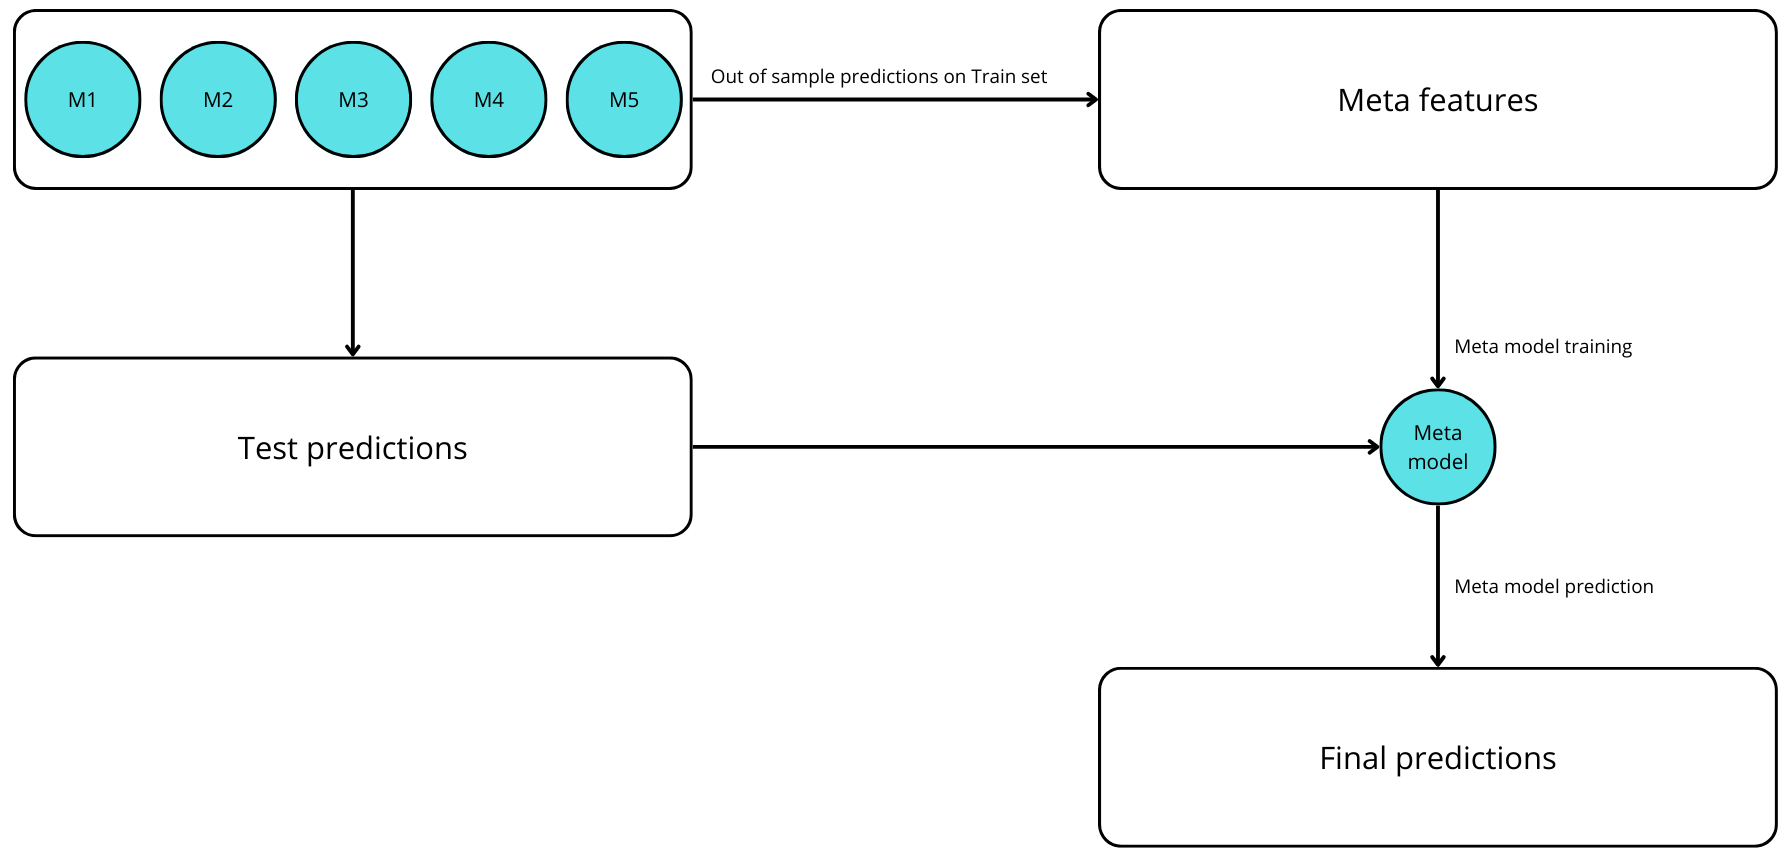
\includegraphics[width=0.7\textwidth]{Machine_learning_thesis/Images/Stacking workflow.png}
    \caption{Stacking workflow.} 
    \label{fig:Stacking workflow}
\end{figure}

\subsubsection{Implementation}
Before deep diving into the results obtained leveraging this technique we'll introduce how the ensemble model was implemented. In the code snippet below we can visualize the implementation of the technique.
\label{stacking implementation}
\begin{lstlisting}[language=Python, caption=Stacking Implementation]
def predict(self):
        #parallel execution
        with ThreadPoolExecutor() as executor: 
            results = list(executor.map(self.k_fold_model_prediction, self.trained_models)) 

        # Combine oof predictions into a single array (meta features)
        self.oof_predictions = np.hstack([item.reshape(-1, 1) for item in results])

        #train meta model
        self.meta_model.fit(self.oof_predictions, self.Robustscaler.inverse_transform(self.y_train[(self.fist_fold_idx -self.window_size):]))

        #retrain model on all train set 
        with ThreadPoolExecutor() as executor: #it creates a pool of worker threads (the with statement ensures that the pool of threads is cleaned up automatically after the execution)
            test_results = list(executor.map(self.model_prediction, self.trained_models)) 

        #stack test predictions
        self.test_predictions = np.hstack([item.reshape(-1, 1) for item in test_results])

        #use meta model to generate final predictions 
        final_preds = self.meta_model.predict(self.test_predictions)

        return final_preds
\end{lstlisting}
The workflow can be summarized by the following steps:
\begin{enumerate}
    \item meta features are computed performing k-fold cross-validation for each base model on the training set, with each fold designed to be time aware, maintaining the temporal order intact.
    \item a meta model is trained, in this particolar implementation a linear regressor was used, but any other meta model can be selected by the user using the library API. 
    \item the base models are retrained on the entire training set to maximize their exposure to historical patterns, and test predictions are computed
    \item the test predictions are stacked and fed into the meta model to produce the final forecast.
\end{enumerate}

\subsubsection{Results}
In the table below are presented the results of the Stacking ensemble technique on both datasets.
\begin{table}[h]
    \centering
    \resizebox{\textwidth}{!}{  % Resizes table to fit the page
    \begin{tabular}{|c|c|c|c|c|c|c|}
        \hline
        Dataset & RMSE & MSE & MAE & R² Score & MAPE & SMAPE \\
        \hline
        S\&P500 & 58.1909 & 3386.1848 & 43.8442 & 0.9925 & 0.0099 & 0.0099 \\ 
        \hline
        eur/usd & 0.0073 & 0.0000540 & 0.0057 & 0.9538 & 0.0053 & 0.0053 \\ 
        \hline
    \end{tabular}
    }
    \caption{Performance metrics Stacking ensemble}
    \label{tab: stacking performance}
\end{table}

\subsection{Weighted average}
\subsubsection{Implementation}
The code snippets below provide a brief overview of the implementation of the ensemble model.
\label{weighted average implementation}
\begin{lstlisting}[language=Python, caption=Stacking Implementation]
def predict(self):

        #k fold train predictions to infer model weights
        if (self.weights == None):
            print("k fold train predictions")
            with ThreadPoolExecutor() as executor:
                k_fold_results = list(executor.map(self.k_fold_model_prediction, self.trained_models)) 

            #stack r2 scores
            r2 = np.hstack([item[1] for item in k_fold_results])
            r2 = torch.tensor(r2, dtype=torch.float32).detach()

            #filter the k best r2
            best_r2, indices = torch.topk(r2, k=self.k, largest=False, sorted=False)

            #normalize r2 scores
            std = best_r2.std(dim=0, keepdim=True) + 1e-8 #for numerical stability (to avoid division by zero)
            mean = best_r2.mean(dim=0, keepdim=True)

            normalized_r2 = (r2 - mean) / std
            print("unmasked normalized errors")
            print(normalized_r2)

            #apply mask
            mask = torch.zeros_like(r2, dtype=torch.bool)
            mask.scatter_(dim=0, index=indices, value=True)
            normalized_r2[~mask] = float('inf')

            #apply softmax
            self.weights = F.softmax(normalized_r2 * self.temperature, dim=0)

            print('weights')

        #retrain model on all train set 
        with ThreadPoolExecutor() as executor: 
            test_results = list(executor.map(self.model_prediction, self.trained_models)) 

        #stack test predictions
        self.test_predictions = np.hstack([item[0].reshape(-1, 1) for item in test_results])

        #weighted average of the predictions
        final_preds = np.average(self.test_predictions, axis=1, weights=self.weights)

        return final_preds
\end{lstlisting}
A simpler weighted average ensemble was implemented to assess the efficacy of dynamic versus static model weighting strategies. The weighted average approach assigns fixed weights to base models, this weight can be either assigned by the user (leveraging domain expertise or prior knowledge of model strengths) or can be inferred automatically by the model if no weights are explicitly provided. The way the weights are determined can be summarized by the following steps:
\begin{enumerate}
    \item the $R^2$ scores of base models is calculated from their k-fold out-of-sample predictions on the training set
    \item the score are normalized 
    \item a softmax function is applied to the normalized score to convert them into weights.
\end{enumerate}

\subsubsection{Results}
In the table below are presented the results of the Stacking ensemble technique on both datasets. The ensemble has been computed by leaving the model weights unspecified, allowing the model to automatically compute them, greater accuracy can be achieved by manually setting each model weights, by exploiting prior knowledge of how each base model will perform.
\begin{table}[h]
    \centering
    \resizebox{\textwidth}{!}{  % Resizes table to fit the page
    \begin{tabular}{|c|c|c|c|c|c|c|}
        \hline
        Dataset & RMSE & MSE & MAE & R² Score & MAPE & SMAPE \\
        \hline
        S\&P500 & 58.3838 & 3408.6715 & 44.6001 & 0.9924 & 0.0100 & 0.0100 \\
        \hline
        eur/usd & 0.0075 & 0.0000569 & 0.0058 & 0.9513 & 0.0054 & 0.0054 \\
        \hline
    \end{tabular}
    }
    \caption{Performance metrics Weighted average ensemble}
    \label{tab: Weighted average performance}
\end{table}

\section{Limitations and Challenges}
